\documentclass[aspectratio=169,10pt]{beamer}

\usepackage[T1]{fontenc}
\usepackage{sourcesanspro}
\usepackage{sourcecodepro}
\usepackage{booktabs}
\usepackage{tabularx}
\usepackage{array}
\usepackage{graphicx}
\usepackage{tikz}
\usepackage{pgfplots}
\usepackage{fontawesome5}
\usetikzlibrary{arrows.meta,positioning,fit,calc,shapes.geometric}
\pgfplotsset{compat=1.18}

\definecolor{ArchInk}{HTML}{20252B}
\definecolor{ArchMuted}{HTML}{59636D}
\definecolor{ArchBlue}{HTML}{1F5F7A}
\definecolor{ArchBlueLight}{HTML}{EAF3F7}
\definecolor{ArchGreen}{HTML}{3D7A57}
\definecolor{ArchGreenLight}{HTML}{EDF6EF}
\definecolor{ArchRed}{HTML}{A42A38}
\definecolor{ArchRedLight}{HTML}{FAECEE}
\definecolor{ArchGold}{HTML}{B47A18}
\definecolor{ArchGoldLight}{HTML}{FBF3E3}
\definecolor{ArchLine}{HTML}{C8D1D8}
\definecolor{ArchPanel}{HTML}{F6F8F9}

\setbeamercolor{normal text}{fg=ArchInk,bg=white}
\setbeamercolor{structure}{fg=ArchBlue}
\setbeamercolor{frametitle}{fg=ArchInk,bg=white}
\setbeamercolor{alerted text}{fg=ArchRed}
\setbeamerfont{title}{size=\fontsize{24}{28}\selectfont,series=\bfseries}
\setbeamerfont{subtitle}{size=\fontsize{12}{15}\selectfont}
\setbeamerfont{frametitle}{size=\fontsize{18}{22}\selectfont,series=\bfseries}
\setbeamerfont{footline}{size=\fontsize{6.8}{8}\selectfont}
\setbeamertemplate{navigation symbols}{}
\setbeamertemplate{itemize item}{\color{ArchBlue}\small$\blacksquare$}
\setbeamertemplate{itemize subitem}{\color{ArchMuted}\scriptsize$\blacktriangleright$}
\setbeamersize{text margin left=0.55cm,text margin right=0.55cm}

\setbeamertemplate{frametitle}{%
  \nointerlineskip
  \begin{beamercolorbox}[wd=\paperwidth,ht=0.72cm,dp=0.13cm,leftskip=0.58cm,rightskip=0.58cm]{frametitle}
    \usebeamerfont{frametitle}\insertframetitle
  \end{beamercolorbox}
  \vspace{-0.08cm}
  \hspace{0.58cm}\color{ArchBlue}\rule{1.15cm}{0.75pt}\color{ArchLine}\rule{\dimexpr\paperwidth-2.31cm\relax}{0.35pt}
  \vspace{0.12cm}
}

\setbeamertemplate{footline}{%
  \leavevmode
  \hbox{%
    \begin{beamercolorbox}[wd=.53\paperwidth,ht=0.31cm,dp=0.12cm,leftskip=0.58cm]{footline}
      \color{ArchMuted}Architecture 2.0 \enspace|\enspace Slide Layout Catalog
    \end{beamercolorbox}%
    \begin{beamercolorbox}[wd=.29\paperwidth,ht=0.31cm,dp=0.12cm]{footline}
      \hfill\color{ArchBlue}\insertsectionhead
    \end{beamercolorbox}%
    \begin{beamercolorbox}[wd=.18\paperwidth,ht=0.31cm,dp=0.12cm,rightskip=0.58cm plus 1fil]{footline}
      \hfill\color{ArchMuted}\insertframenumber
    \end{beamercolorbox}%
  }
}

\newcommand{\claim}[1]{%
  \begin{beamercolorbox}[rounded=true,sep=0.12cm,wd=\linewidth]{block body}
    \color{ArchBlue}\bfseries #1
  \end{beamercolorbox}\vspace{0.12cm}
}
\newcommand{\source}[1]{%
  \vfill{\fontsize{5.8}{7}\selectfont\color{ArchMuted}Source: #1\par}
}
\newcommand{\tagbox}[3]{%
  \begin{tikzpicture}[baseline=(n.base)]
    \node[rounded corners=2pt,fill=#1,draw=#2,inner xsep=5pt,inner ysep=3pt,
      text=ArchInk,font=\small\bfseries] (n) {#3};
  \end{tikzpicture}
}
\newcommand{\bigsep}[1]{%
  \begin{center}
    \begin{tikzpicture}
      \node[rounded corners=3pt,fill=ArchBlueLight,draw=ArchBlue,
        text width=13.8cm,align=center,minimum height=1.0cm,
        font=\fontsize{15}{19}\selectfont\bfseries,text=ArchBlue] {#1};
    \end{tikzpicture}
  \end{center}
}

\title{Slide Design System \& Layout Catalog}
\subtitle{Standard Arrangements for Architecture 2.0 Presentations}
\author{Architecture 2.0 Design System}
\date{}

\begin{document}

% Slide 1: Cover
\begin{frame}[plain]
  \begin{tikzpicture}[remember picture,overlay]
    \fill[ArchBlue] (current page.north west) rectangle ([xshift=0.14cm]current page.south west);
  \end{tikzpicture}
  \vspace{0.55cm}
  {\color{ArchMuted}\small SLIDE DESIGN SYSTEM\par}
  \vspace{0.35cm}
  {\usebeamerfont{title}\color{ArchInk}\inserttitle\par}
  \vspace{0.12cm}
  {\usebeamerfont{subtitle}\color{ArchMuted}\insertsubtitle\par}
  \vspace{0.45cm}
  \begin{center}
    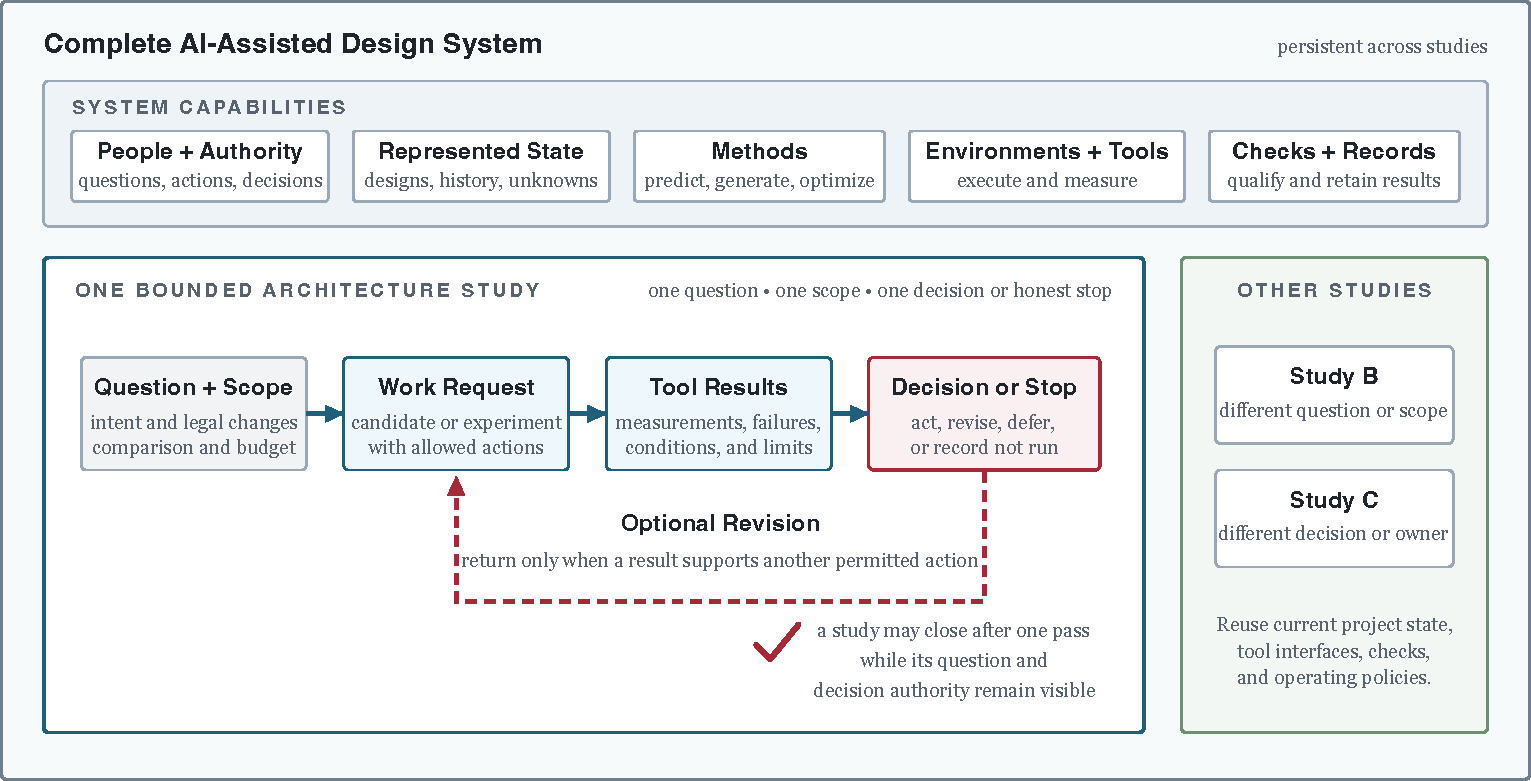
\includegraphics[width=0.72\linewidth,height=3.35cm,keepaspectratio]{../book/images/arch2-loop-diagram.pdf}
  \end{center}
  \vfill
  {\small\color{ArchInk}Three Canonical Archetypes: Plot Only, Plot with Side Text, Just Text\hfill\color{ArchMuted}arch2.mlsysbook.ai\par}
\end{frame}

\section{Catalog}

% Slide 2: Archetype 1: Plot only
\begin{frame}{Archetype 1: A plot only}
  \claim{Use when the graphic is self-contained and visually rich, allowing the speaker to unpack details orally without competing text.}
  \begin{center}
    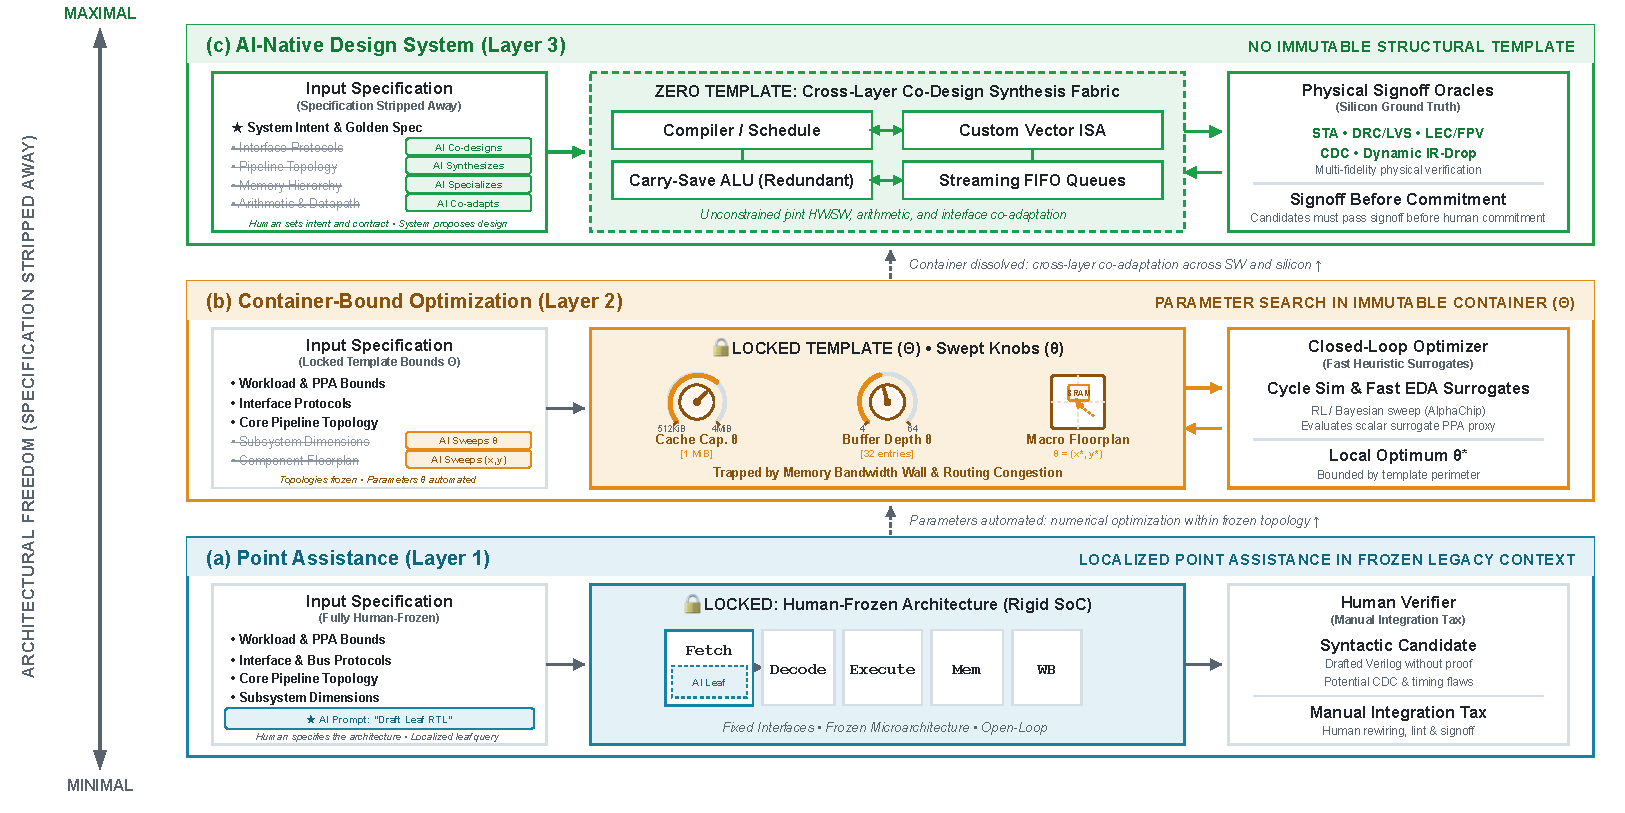
\includegraphics[width=0.96\linewidth,height=4.50cm,keepaspectratio]{../book/contents/chapters/01-moonshot/images/fig-ch01-three-layers-ai-integration.pdf}
  \end{center}
  \source{Architecture 2.0, Chapter 1; Section 1.3. Ideal for keynotes, dense timelines, scaling frontiers, and architecture topologies.}
\end{frame}

% Slide 3: Archetype 2: Plot with text on the side
\begin{frame}{Archetype 2: Plot with text on the side}
  \claim{Use when a diagram requires immediate domain contextualization, takeaway badges, or explicit constraint items alongside the graphic.}
  \begin{columns}[c,onlytextwidth]
    \column{0.64\textwidth}
      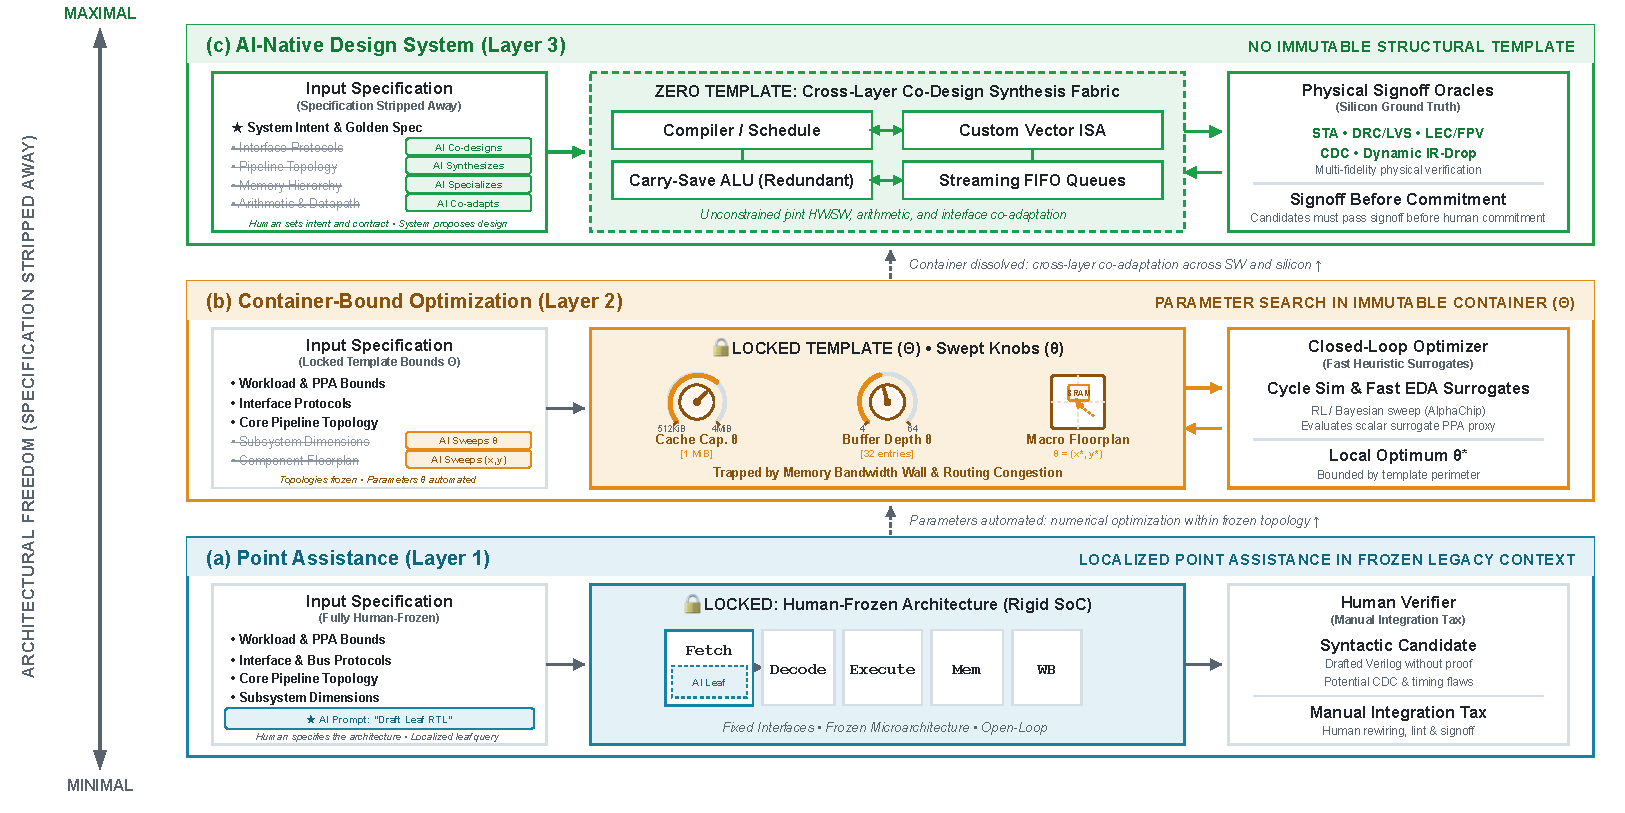
\includegraphics[width=\linewidth,height=4.65cm,keepaspectratio]{../book/contents/chapters/01-moonshot/images/fig-ch01-three-layers-ai-integration.pdf}
    \column{0.33\textwidth}
      \tagbox{ArchBlueLight}{ArchBlue}{Layer 1: AI-Assisted}
      \vspace{0.08cm}
      \begin{itemize}\setlength{\itemsep}{1pt}\small
        \item Point syntax in frozen RTL
        \item Open-loop human review
      \end{itemize}
      \vspace{0.14cm}
      \tagbox{ArchGoldLight}{ArchGold}{Layer 2: AI-Driven}
      \vspace{0.08cm}
      \begin{itemize}\setlength{\itemsep}{1pt}\small
        \item Parameter search $\theta \in \Theta$
        \item Locked container; surrogates
      \end{itemize}
      \vspace{0.14cm}
      \tagbox{ArchGreenLight}{ArchGreen}{Layer 3: AI-Native}
      \vspace{0.08cm}
      \begin{itemize}\setlength{\itemsep}{1pt}\small
        \item Zero structural template
        \item Closed-loop physical signoff
      \end{itemize}
  \end{columns}
  \source{Architecture 2.0, Chapter 1; Section 1.3. Ideal for lecture slides, teaching concepts, and guided visual walkthroughs.}
\end{frame}

% Slide 4: Archetype 3a: Just text - Comparative Card Grid
\begin{frame}{Archetype 3a: Just text (Comparative card grid)}
  \claim{Use for multi-dimensional criteria or tradeoffs, grouping insights into balanced, color-coded thematic columns.}
  \vspace{0.15cm}
  \begin{columns}[T,onlytextwidth]
    \column{0.31\textwidth}
      \tagbox{ArchBlueLight}{ArchBlue}{Architecture quality}
      \vspace{0.15cm}
      \begin{itemize}\setlength{\itemsep}{3pt}
        \item Performance, power, and area
        \item Thermal and reliability limits
        \item Software and compiler fit
      \end{itemize}
    \column{0.31\textwidth}
      \tagbox{ArchGreenLight}{ArchGreen}{Total cost}
      \vspace{0.15cm}
      \begin{itemize}\setlength{\itemsep}{3pt}
        \item Model inference and tokens
        \item EDA license server queue time
        \item Human review and triage effort
      \end{itemize}
    \column{0.31\textwidth}
      \tagbox{ArchRedLight}{ArchRed}{Failure behavior}
      \vspace{0.15cm}
      \begin{itemize}\setlength{\itemsep}{3pt}
        \item Non-synthesizable candidates
        \item Silent constraint tampering
        \item Unsafe or uncontrolled actions
      \end{itemize}
  \end{columns}
  \source{Architecture 2.0, Chapter 1; The Architecture 2.0 Bet.}
\end{frame}

% Slide 5: Archetype 3b: Just text - Decision Flow & Alert Constraints
\begin{frame}{Archetype 3b: Just text (Decision flow \& alerts)}
  \claim{Use to establish sequential evaluation gates, formal handoffs, or boundary conditions across an end-to-end workflow.}
  \vspace{0.25cm}
  \begin{center}
  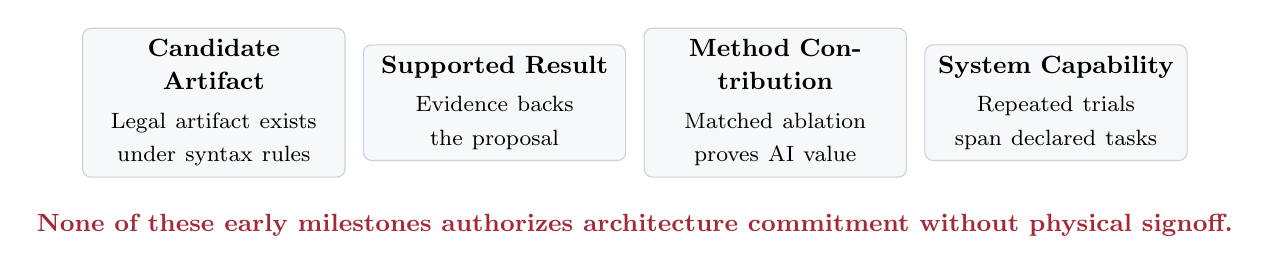
\begin{tikzpicture}[node distance=0.22cm]
    \tikzset{claimstep/.style={rounded corners=3pt,draw=ArchLine,fill=ArchPanel,
      text width=3.05cm,minimum height=1.45cm,align=center,inner sep=4pt}}
    \node[claimstep] (a) {{\small\bfseries Candidate Artifact}\\[2pt]{\footnotesize Legal artifact exists under syntax rules}};
    \node[claimstep,right=of a] (b) {{\small\bfseries Supported Result}\\[2pt]{\footnotesize Evidence backs the proposal}};
    \node[claimstep,right=of b] (c) {{\small\bfseries Method Contribution}\\[2pt]{\footnotesize Matched ablation proves AI value}};
    \node[claimstep,right=of c] (d) {{\small\bfseries System Capability}\\[2pt]{\footnotesize Repeated trials span declared tasks}};
    \node[below=0.45cm of $(b.south)!0.5!(c.south)$,align=center,text=ArchRed,font=\small\bfseries]
      {None of these early milestones authorizes architecture commitment without physical signoff.};
  \end{tikzpicture}
  \end{center}
  \source{Architecture 2.0, Chapter 1; Four Distinct Success Claims.}
\end{frame}

% Slide 6: Archetype 3c: Just text - Big Thesis / Contrast Banner
\begin{frame}{Archetype 3c: Just text (The big thesis banner)}
  \claim{Use to establish an authoritative axiom, counter-intuitive insight, or keynote turning point.}
  \vspace{0.25cm}
  \bigsep{A foundation model does not design a chip.\\The surrounding verification harness designs the chip.}
  \vspace{0.25cm}
  \begin{columns}[T,onlytextwidth]
    \column{0.46\textwidth}
      \tagbox{ArchRedLight}{ArchRed}{The Common Assumption}
      \vspace{0.15cm}
      \begin{itemize}
        \item Generative models replace engineers by emitting raw RTL text in isolation.
      \end{itemize}
    \column{0.46\textwidth}
      \tagbox{ArchGreenLight}{ArchGreen}{The Architectural Reality}
      \vspace{0.15cm}
      \begin{itemize}
        \item Value is created when physical signoff oracles bound and guide the search space.
      \end{itemize}
  \end{columns}
  \source{Architecture 2.0, Chapter 1; Core Thesis.}
\end{frame}

\end{document}
